\chapter{Higher Level Behavior Modeling}

In this chapter, we first discuss the relationships between user's lower level and higher level behavior in web search background. This is a prelude for the rest of this chapter. We are intended to deal with the process of modeling user's higher abstraction level behavior and its implementation. 

Our first task was to understand the space of user goals. In particular, we needed to come up with a framework that could identify and organize a manageable set of canonical goal categories. These goal categories, in turn, must encompass the majority of actual goals users have in mind when searching.

\section{Relationships of Lower Level and Higher Level Behavior}

In the web era, search engines are used for more than just research. Even the most cursory look at the query logs of many major search engine makes it clear that the goal underlying web searches are many and varied. And while the vast body of work described above has helped us to understand {\it what} users are searching for and {\it how} their information-seeking process works, there have been few attempts to look at {\it why} users are searching.

One of the fear exceptions is Broder's ``Taxonomy of Web Search''\cite{Broder2002}. Motivated by the idea that the traditional notion of an ``information need'' might not adequately describe web searching, Broder came up with a trichotomy of web search ``types'': {\bf navigational}, {\bf informational}, and {\bf transactional}. {\it Navigational} searches are those which are intended to find a specific web site that the user has in mind; {\it informational} searches are intended to find information about a topic; {\it transactional} searches are intended to ``perform some web-mediated activity''.

User's interests change over time, studies of user search behavior have a long history in Information and Library Science\cite{Bates1979}\cite{Rose}\cite{Spink2002}. When a user browses the web at different times, she could be accessing pages that pertain to different topics. For example, a user might be looking for research papers at one time and airfare information for conference travel at another. That is, a user can exhibit different kinds of interests at different times, which provides different contexts underlying a user's behavior. However, different kinds of interests might be motivated by the same kind of interest at a higher abstraction level. That is, a user might posse interests at different abstraction level - the higher level interests are more general, while the lower-level ones are more specific.

In order to definitively know the underlying goal of every user query, we would need to be able to ask the user about her interest. Clearly, this is not feasible in most cases\cite{Marchionini2006}. But can the goal be determined simply by looking at the query itself, or is more information required? During a browse session, general interests are in the back of one's mind, while specific interests are the current foci. In this paper, we focus on implicit methods for incremental creating an ordered representation of user profiles. Utilizing an interest score, has been proven to be successful for the evolution of personal interest \cite{Sieg2007}. 

\section{Traditional Faceted Search}

In the traditional faceted search, each category is represented by a facet, user can choose different facets to drill down the search results. A screen shot of the classical faceted search is shown in Figure 2.1. Unlike document-based relevance feedback mechanism which asks users to give feedback on the relevance of documents. Faceted search allows users to give feedback on document metadata fields.

As a motivate example, let us consider a scenario that an user wants to find a restaurant where is near by a famous place she might want to visit after lunch. To find the most suitable restaurant, she needs to first search for a restaurant then clicks on different facets to filter the searched result. Multiple clicks present her interest score, however unless she could construct a complicated query, she could not easily represent her interest.

\begin{figure}
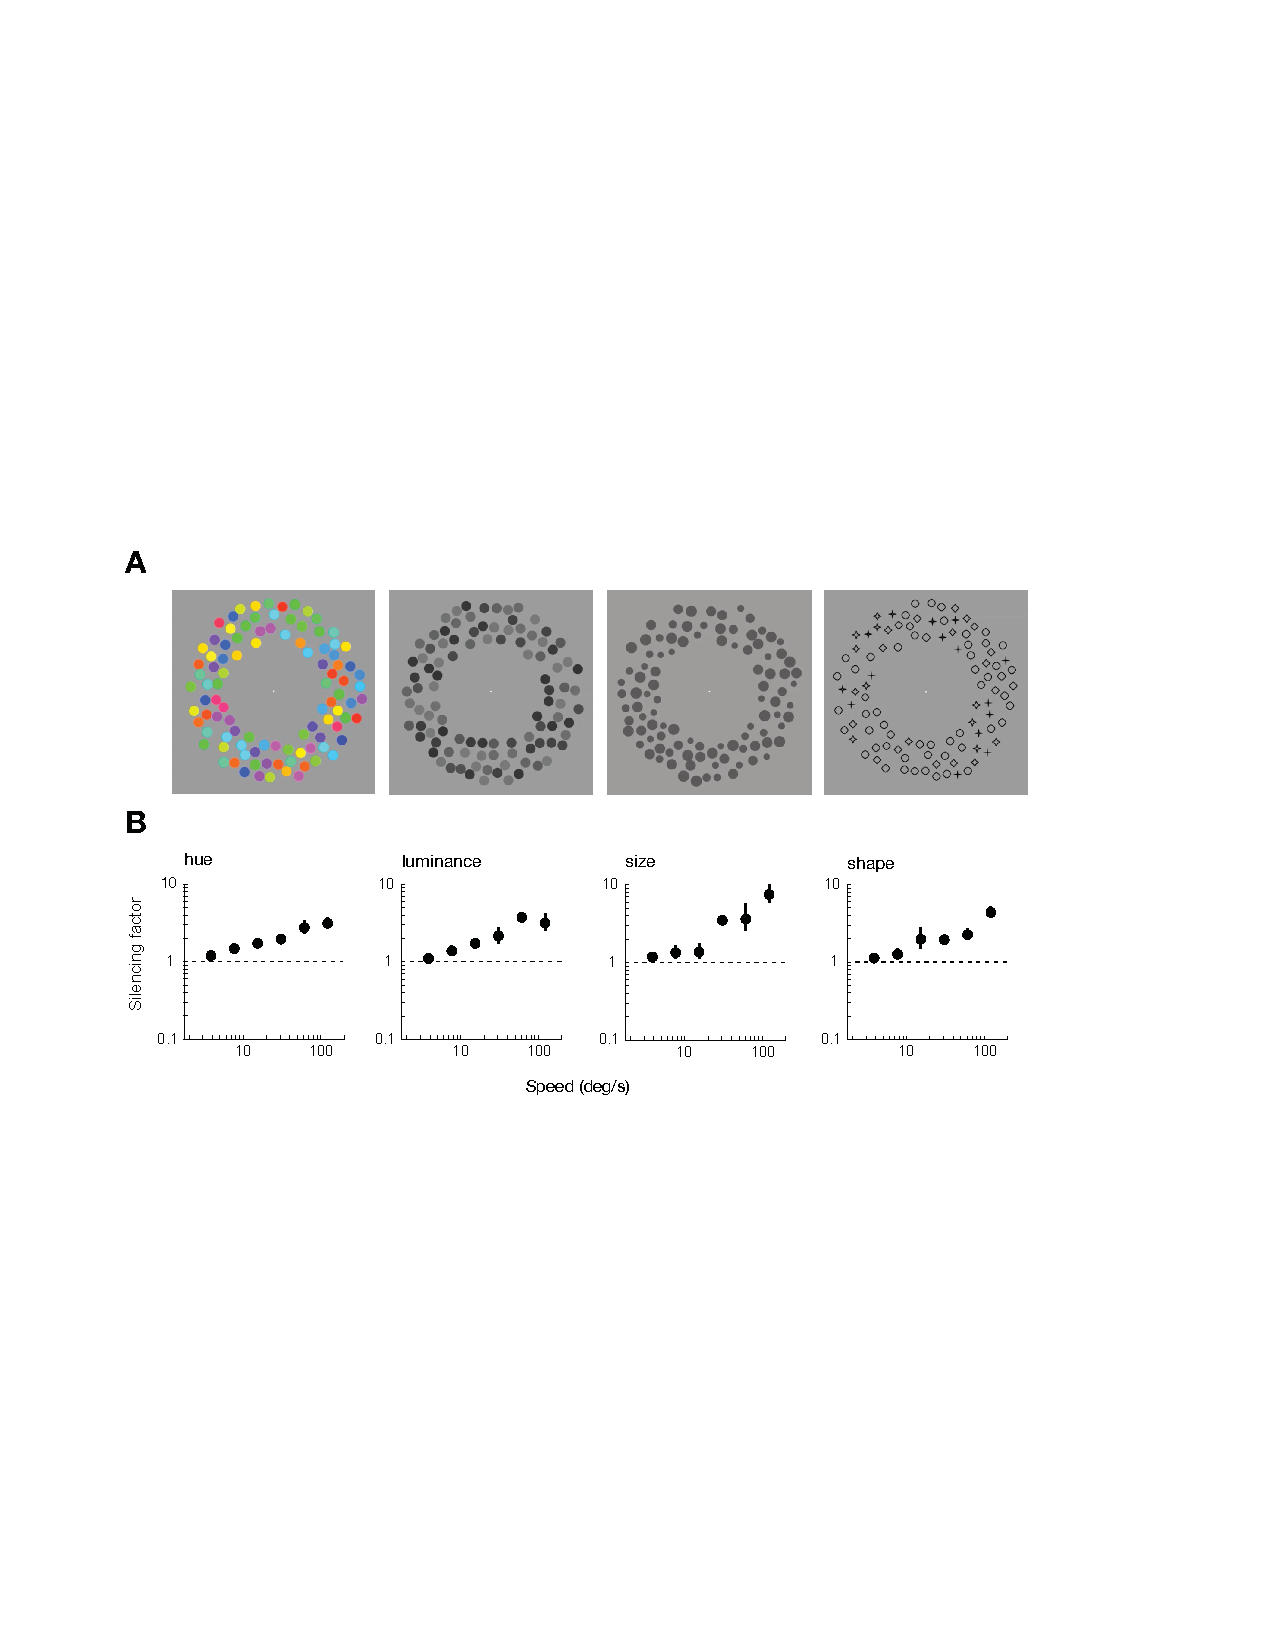
\includegraphics[width=\textwidth]{figures/fig1}
\caption[Traditional Faceted Search.]{A screen shot of traditional faceted search.
\label{fig:myInlineFigure}}
\end{figure}

\section{Hits Queue Model for Facets}

This common scenario inspires us to map user's clicks into a {\it Hits Queue}. In this paper, each metadata field is called a facet, and a facet ({\it f}) with a specific value ({\it v}) is called a facet-value pair ({\it f : v}). Each facet-value pair represents a faceted constraint on returned documents, E.g., language:Chinese, format:ppt: subject:IR, genre:comedy.

To void overwhelming users with many facet-value pair candidates, the system needs to recommend a small number of facet-value pairs that are most probably interesting to a user. A good recommendation approach is crucial in the faceted feedback mechanism. Intuitively, the recommended facet-value pair should be good in - they have a high score of being relevant and thus chosen by the user. Based on this respect, we propose {\it Top Document Score (TDS)} method. 

To select the most frequent facet-value pairs occurring in the top {\it N} ranked documents returned by a baseline retrieval algorithm using the initial query. We calculate the interest score instead of frequency of each face-value pair in the top {\it N} documents, which is called ``Top {\it N} Document Score''. The top {\it N} most highest score facet-value pairs are chosen as candidates to present to the user. The underlying data structure of {\it Hits Queue} is a priority queue. A priority queue is a queue for which each element has an associated priority, and for which the dequeue operation always removes the lowest (or highest) priority item remaining in the queue. 

\section{Mapping clicks to Hits Queue}

A chosen {\it f}  is presented by a facet in the priority queue. A {\it priority} contains a set of facet-value pair {\it f: v}. To map facet-value pairs, the hits queue is generated with the interaction processing while the user clicking on different facets. As user dynamically change their preferences during the time, the hits queue . Furthermore, the number of hits, when clicking for the entity, is stored as {\it freq(md)}. We construct the queue from users clicks as follows:

\begin{itemize}
    \item Initialize each facet as {\it {f: 0}}.
    \item User clicks on a certain facet she is interested in.
    \item Improve this facet's score by 1, it becomes to the first node in the queue.
    \item User clicks on another facet.
    \item Reorder the queue with different priority. \ldots
\end{itemize}

The motivation of using {\it Hits Queue} is twofold: 1) a facet-value pair that appears rarely in the whole corpus while frequently in top ranked documents has a high probability to be relevant; 2) the retrieval system gets more benefits by knowing a rare facet-value pair covering a small number of documents being relevant that a frequent one.
